\documentclass[xelatex, ja=standard, b5paper]{bxjsbook}
\usepackage{lmodern}
\usepackage{amssymb,amsmath}
\usepackage{ifxetex,ifluatex}
\usepackage{fixltx2e} % provides \textsubscript
\ifnum 0\ifxetex 1\fi\ifluatex 1\fi=0 % if pdftex
  \usepackage[T1]{fontenc}
  \usepackage[utf8]{inputenc}
\else % if luatex or xelatex
  \ifxetex
    \usepackage{mathspec}
  \else
    \usepackage{fontspec}
  \fi
  \defaultfontfeatures{Ligatures=TeX,Scale=MatchLowercase}
\fi
% use upquote if available, for straight quotes in verbatim environments
\IfFileExists{upquote.sty}{\usepackage{upquote}}{}
% use microtype if available
\IfFileExists{microtype.sty}{%
\usepackage{microtype}
\UseMicrotypeSet[protrusion]{basicmath} % disable protrusion for tt fonts
}{}
% \usepackage[no]{geometry}
\usepackage{hyperref}
\hypersetup{unicode=true,
            pdftitle={bookdownの体験},
            pdfauthor={izunyan},
            pdfborder={0 0 0},
            breaklinks=true}
\urlstyle{same}  % don't use monospace font for urls
\usepackage{color}
\usepackage{fancyvrb}
\newcommand{\VerbBar}{|}
\newcommand{\VERB}{\Verb[commandchars=\\\{\}]}
\DefineVerbatimEnvironment{Highlighting}{Verbatim}{commandchars=\\\{\}}
% Add ',fontsize=\small' for more characters per line
\usepackage{framed}
\definecolor{shadecolor}{RGB}{248,248,248}
\newenvironment{Shaded}{\begin{snugshade}}{\end{snugshade}}
\newcommand{\AlertTok}[1]{\textcolor[rgb]{0.94,0.16,0.16}{#1}}
\newcommand{\AnnotationTok}[1]{\textcolor[rgb]{0.56,0.35,0.01}{\textbf{\textit{#1}}}}
\newcommand{\AttributeTok}[1]{\textcolor[rgb]{0.77,0.63,0.00}{#1}}
\newcommand{\BaseNTok}[1]{\textcolor[rgb]{0.00,0.00,0.81}{#1}}
\newcommand{\BuiltInTok}[1]{#1}
\newcommand{\CharTok}[1]{\textcolor[rgb]{0.31,0.60,0.02}{#1}}
\newcommand{\CommentTok}[1]{\textcolor[rgb]{0.56,0.35,0.01}{\textit{#1}}}
\newcommand{\CommentVarTok}[1]{\textcolor[rgb]{0.56,0.35,0.01}{\textbf{\textit{#1}}}}
\newcommand{\ConstantTok}[1]{\textcolor[rgb]{0.00,0.00,0.00}{#1}}
\newcommand{\ControlFlowTok}[1]{\textcolor[rgb]{0.13,0.29,0.53}{\textbf{#1}}}
\newcommand{\DataTypeTok}[1]{\textcolor[rgb]{0.13,0.29,0.53}{#1}}
\newcommand{\DecValTok}[1]{\textcolor[rgb]{0.00,0.00,0.81}{#1}}
\newcommand{\DocumentationTok}[1]{\textcolor[rgb]{0.56,0.35,0.01}{\textbf{\textit{#1}}}}
\newcommand{\ErrorTok}[1]{\textcolor[rgb]{0.64,0.00,0.00}{\textbf{#1}}}
\newcommand{\ExtensionTok}[1]{#1}
\newcommand{\FloatTok}[1]{\textcolor[rgb]{0.00,0.00,0.81}{#1}}
\newcommand{\FunctionTok}[1]{\textcolor[rgb]{0.00,0.00,0.00}{#1}}
\newcommand{\ImportTok}[1]{#1}
\newcommand{\InformationTok}[1]{\textcolor[rgb]{0.56,0.35,0.01}{\textbf{\textit{#1}}}}
\newcommand{\KeywordTok}[1]{\textcolor[rgb]{0.13,0.29,0.53}{\textbf{#1}}}
\newcommand{\NormalTok}[1]{#1}
\newcommand{\OperatorTok}[1]{\textcolor[rgb]{0.81,0.36,0.00}{\textbf{#1}}}
\newcommand{\OtherTok}[1]{\textcolor[rgb]{0.56,0.35,0.01}{#1}}
\newcommand{\PreprocessorTok}[1]{\textcolor[rgb]{0.56,0.35,0.01}{\textit{#1}}}
\newcommand{\RegionMarkerTok}[1]{#1}
\newcommand{\SpecialCharTok}[1]{\textcolor[rgb]{0.00,0.00,0.00}{#1}}
\newcommand{\SpecialStringTok}[1]{\textcolor[rgb]{0.31,0.60,0.02}{#1}}
\newcommand{\StringTok}[1]{\textcolor[rgb]{0.31,0.60,0.02}{#1}}
\newcommand{\VariableTok}[1]{\textcolor[rgb]{0.00,0.00,0.00}{#1}}
\newcommand{\VerbatimStringTok}[1]{\textcolor[rgb]{0.31,0.60,0.02}{#1}}
\newcommand{\WarningTok}[1]{\textcolor[rgb]{0.56,0.35,0.01}{\textbf{\textit{#1}}}}
\usepackage{longtable,booktabs}
\usepackage{graphicx,grffile}
\makeatletter
\def\maxwidth{\ifdim\Gin@nat@width>\linewidth\linewidth\else\Gin@nat@width\fi}
\def\maxheight{\ifdim\Gin@nat@height>\textheight\textheight\else\Gin@nat@height\fi}
\makeatother
% Scale images if necessary, so that they will not overflow the page
% margins by default, and it is still possible to overwrite the defaults
% using explicit options in \includegraphics[width, height, ...]{}
\setkeys{Gin}{width=\maxwidth,height=\maxheight,keepaspectratio}
\usepackage[normalem]{ulem}
% avoid problems with \sout in headers with hyperref:
\pdfstringdefDisableCommands{\renewcommand{\sout}{}}
\IfFileExists{parskip.sty}{%
\usepackage{parskip}
}{% else
\setlength{\parindent}{0pt}
\setlength{\parskip}{6pt plus 2pt minus 1pt}
}
\setlength{\emergencystretch}{3em}  % prevent overfull lines
\providecommand{\tightlist}{%
  \setlength{\itemsep}{0pt}\setlength{\parskip}{0pt}}
\setcounter{secnumdepth}{5}
% Redefines (sub)paragraphs to behave more like sections
\ifx\paragraph\undefined\else
\let\oldparagraph\paragraph
\renewcommand{\paragraph}[1]{\oldparagraph{#1}\mbox{}}
\fi
\ifx\subparagraph\undefined\else
\let\oldsubparagraph\subparagraph
\renewcommand{\subparagraph}[1]{\oldsubparagraph{#1}\mbox{}}
\fi

%%% Use protect on footnotes to avoid problems with footnotes in titles
\let\rmarkdownfootnote\footnote%
\def\footnote{\protect\rmarkdownfootnote}

%%% Change title format to be more compact
\usepackage{titling}

% Create subtitle command for use in maketitle
\providecommand{\subtitle}[1]{
  \posttitle{
    \begin{center}\large#1\end{center}
    }
}

\setlength{\droptitle}{-2em}

  \title{bookdownの体験}
    \pretitle{\vspace{\droptitle}\centering\huge}
  \posttitle{\par}
    \author{izunyan}
    \preauthor{\centering\large\emph}
  \postauthor{\par}
    \date{}
    \predate{}\postdate{}
  

\begin{document}
\maketitle

{
\setcounter{tocdepth}{1}
\tableofcontents
}
\hypertarget{hajime}{%
\chapter*{はじめに}\label{hajime}}
\addcontentsline{toc}{chapter}{はじめに}


\includegraphics[width=0.6\linewidth]{images/cover}

(2019/11/10現在)

\begin{itemize}
\item
  何も考えずにとりあえずbookdownでファイルを作ってみる
\item
  bookdownで作られた有名な例

  \begin{itemize}
  \tightlist
  \item
    \href{https://r4ds.had.co.nz/}{R for Data Science}
  \item
    \href{https://github.com/hadley/r4ds}{元のマークダウンファイルなど}
  \end{itemize}
\item
  詳しくは公式ドキュメント参照

  \begin{itemize}
  \tightlist
  \item
    \href{https://bookdown.org/yihui/bookdown/}{bookdown: Authoring Books and Technical Documents with R Markdown}
  \item
    \href{https://github.com/rstudio/bookdown/tree/master/inst/examples}{元のマークダウンファイルなど}
  \end{itemize}
\end{itemize}

\hypertarget{hajime_dl}{%
\section*{サンプルの最小構成プロジェクトをダウンロード}\label{hajime_dl}}
\addcontentsline{toc}{section}{サンプルの最小構成プロジェクトをダウンロード}

\begin{Shaded}
\begin{Highlighting}[]
\CommentTok{# パッケージが入っていない方はまずインストール}
\KeywordTok{install.packages}\NormalTok{(}\StringTok{"bookdown"}\NormalTok{)}
\end{Highlighting}
\end{Shaded}

\url{https://github.com/yihui/bookdown-minimal}

の

Clone or download \textgreater{} Download ZIP

でダウンロードしたファイルを解凍する



\begin{figure}

{\centering \includegraphics[width=0.7\linewidth]{images/github} 

}

\caption{Clone or downloadの場所}\label{fig:github}
\end{figure}

\hypertarget{hajime_open}{%
\section*{プロジェクトファイルを開く}\label{hajime_open}}
\addcontentsline{toc}{section}{プロジェクトファイルを開く}

解凍したフォルダ内のプロジェクトファイル\texttt{bookdown-minimal.Rproj} を実行

\hypertarget{hajime_bb}{%
\section*{Build Bookする}\label{hajime_bb}}
\addcontentsline{toc}{section}{Build Bookする}

右上ペインのBuildタブを開き,\texttt{Build\ Book}を押す



\begin{figure}

{\centering \includegraphics[width=0.7\linewidth]{images/migiue} 

}

\caption{Build Bookの場所}\label{fig:migiue}
\end{figure}

\begin{itemize}
\tightlist
\item
  ここまでで最小構成版は完成。ここの時点ではまだ\texttt{\_bookdown.yml}や\texttt{\_output.yml}はなくても大丈夫みたい
\end{itemize}

\hypertarget{hajime_add}{%
\section*{最小構成から色々追加していくために}\label{hajime_add}}
\addcontentsline{toc}{section}{最小構成から色々追加していくために}

\begin{itemize}
\tightlist
\item
  \protect\hyperlink{intro}{1 章の追加}からを参照
\item
  追加される章のrmdファイルの順番や,必要なフォルダ名の命名のため等に\texttt{\_bookdown.yml}の作成が必要
\end{itemize}

\hypertarget{intro}{%
\chapter{章の追加}\label{intro}}

\begin{itemize}
\tightlist
\item
  新しいRmdファイルを作成
\item
  \sout{名前は「数値\_ファイル名」にしてみた(よりよいつけ方は勉強中)}
\item
  数値\_ファイル名だと,後から章を挿入するときに不便なので,\texttt{\_bookdown.yml}にて\texttt{rmd\_files:\ {[}{]}}中に並べたい順に指定
\item
  ここから1章として始める(はじめにの章に数字をつけない)ためには,index.Rmdのヘッダーの後に \texttt{\{-\}}をつける

  \begin{itemize}
  \tightlist
  \item
    参照:\url{https://bookdown.org/yihui/bookdown/markdown-syntax.html\#block-level-elements}
  \item
    ただし,エラー回避のため,漢字が含まれるヘッダーについて,識別子(例:\texttt{\{-\#hajimeni\}})をつけている
  \end{itemize}
\end{itemize}

\hypertarget{intro_link}{%
\section{テキスト内のリンク}\label{intro_link}}

\begin{itemize}
\tightlist
\item
  まず4章見出し部分の記述を\texttt{\#\ 参考サイト\ \{\#sanko\}}としておく
\item
  章の数字でリンクを張る:\ref{sanko}章。左のリンク部分は\texttt{\textbackslash{}@ref(sanko)}と記述
\item
  章の名前でリンクを張る:
  \protect\hyperlink{sanko}{参考サイト}。左のリンク部分は\texttt{{[}参考サイト{]}(\#sanko)}と記述
\end{itemize}

\hypertarget{intro_sansho}{%
\section{図の参照}\label{intro_sansho}}

\begin{itemize}
\tightlist
\item
  Figure\ref{fig:irisplot}にとぶ。左のリンク部分は\texttt{\textbackslash{}@ref(fig:irisplot)}と記述
\end{itemize}

\hypertarget{figure}{%
\chapter{図}\label{figure}}

\hypertarget{figure_fig}{%
\section{図}\label{figure_fig}}

\begin{itemize}
\tightlist
\item
  図の名前の指定\texttt{(ref:irisplot)\ 図のタイトル}
\end{itemize}



\begin{Shaded}
\begin{Highlighting}[]
\KeywordTok{plot}\NormalTok{(iris}\OperatorTok{$}\NormalTok{Sepal.Length, iris}\OperatorTok{$}\NormalTok{Petal.Length)}
\end{Highlighting}
\end{Shaded}

\begin{figure}

{\centering 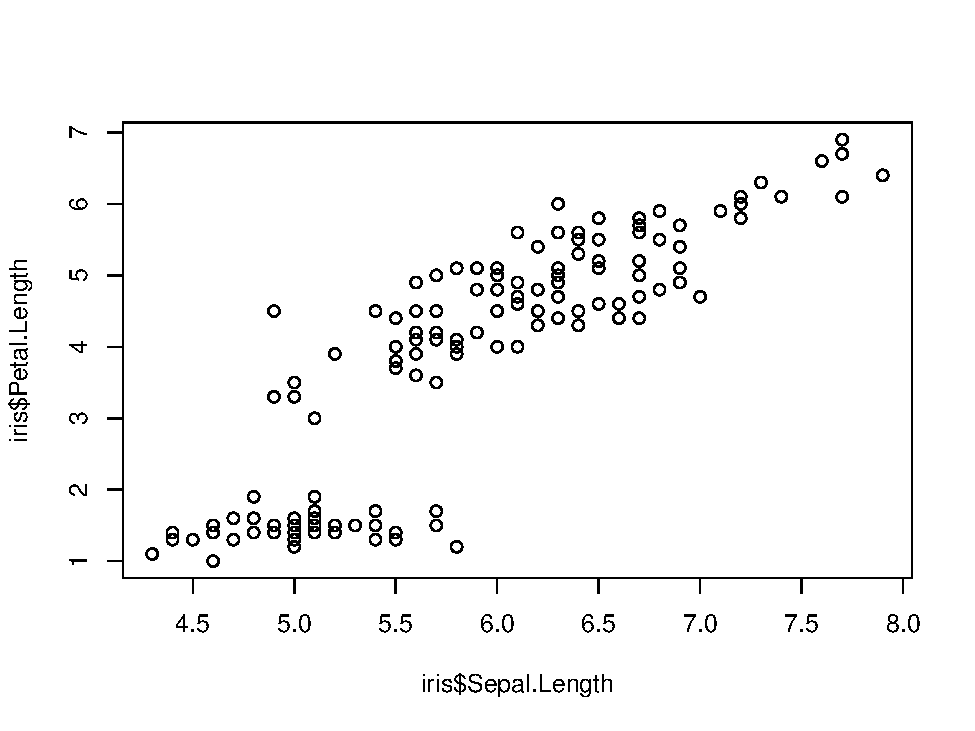
\includegraphics[width=0.7\linewidth]{bookdown_taiken_files/figure-latex/irisplot-1} 

}

\caption{図のタイトル}\label{fig:irisplot}
\end{figure}



\begin{Shaded}
\begin{Highlighting}[]
\KeywordTok{library}\NormalTok{(tidyverse)}
\end{Highlighting}
\end{Shaded}

\begin{Shaded}
\begin{Highlighting}[]
\KeywordTok{ggplot}\NormalTok{(iris) }\OperatorTok{+}
\StringTok{  }\KeywordTok{geom_point}\NormalTok{(}\KeywordTok{aes}\NormalTok{(Sepal.Length, Petal.Length, }\DataTypeTok{color =}\NormalTok{ Species))}
\end{Highlighting}
\end{Shaded}

\begin{figure}

{\centering 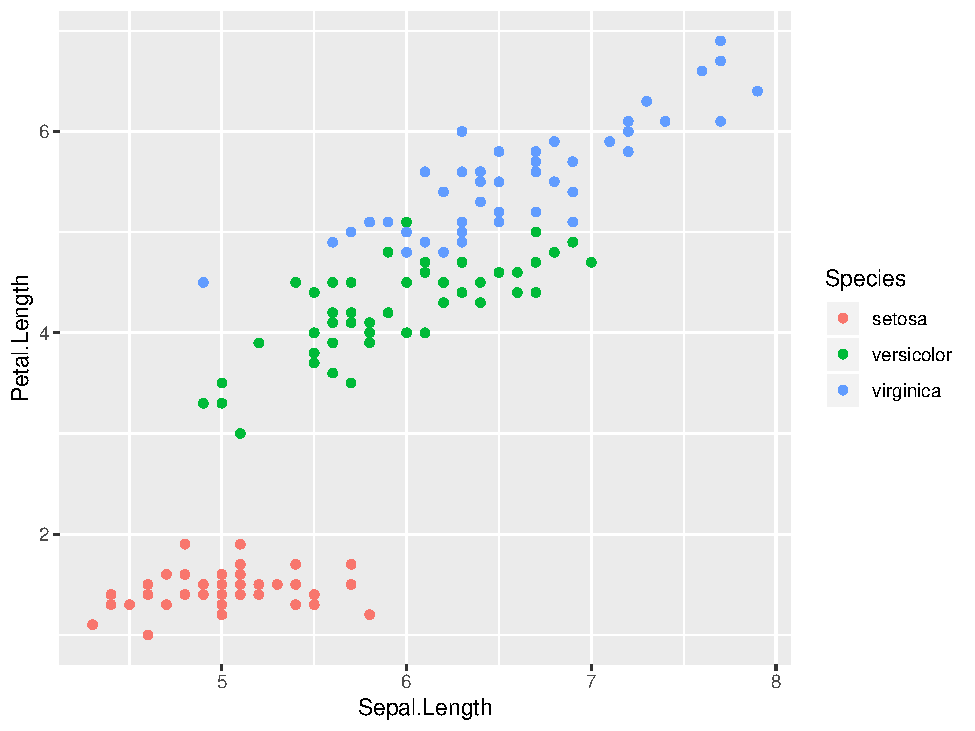
\includegraphics[width=0.7\linewidth]{bookdown_taiken_files/figure-latex/iris-ggplot-1} 

}

\caption{ggplot}\label{fig:iris-ggplot}
\end{figure}

\sout{図が出ない(T\_T)}\\
→解決!

\begin{itemize}
\tightlist
\item
  考えられる理由

  \begin{itemize}
  \tightlist
  \item
    \texttt{bookdown.yml}中の\texttt{book\_filename:}のところの名前に日本語を使っていたため。これはコード実行して作成される図のファイルが入る\texttt{\_bookdown\_files}の中のフォルダ名になるようで,日本語だとパスが読めずこの図が表示されない事が起こる。
  \item
    そもそも\texttt{docs}フォルダ内に\texttt{book\_filename:}で指定される名前のフォルダが自動作成されるみたいで,日本語だとこれ自体が作成されなかった
  \end{itemize}
\end{itemize}

\hypertarget{figure_table}{%
\section{表}\label{figure_table}}

\begin{Shaded}
\begin{Highlighting}[]
\NormalTok{knitr}\OperatorTok{::}\KeywordTok{kable}\NormalTok{(}
  \KeywordTok{head}\NormalTok{(mtcars[, }\DecValTok{1}\OperatorTok{:}\DecValTok{3}\NormalTok{], }\DecValTok{5}\NormalTok{), }\DataTypeTok{booktabs =} \OtherTok{TRUE}\NormalTok{, }\CommentTok{# 1-3列目のみ,最初の5行}
  \DataTypeTok{caption =} \StringTok{'mtcarsデータの最初の5行の表'}
\NormalTok{)}
\end{Highlighting}
\end{Shaded}

\begin{table}

\caption{\label{tab:table-mtcar}mtcarsデータの最初の5行の表}
\centering
\begin{tabular}[t]{lrrr}
\toprule
  & mpg & cyl & disp\\
\midrule
Mazda RX4 & 21.0 & 6 & 160\\
Mazda RX4 Wag & 21.0 & 6 & 160\\
Datsun 710 & 22.8 & 4 & 108\\
Hornet 4 Drive & 21.4 & 6 & 258\\
Hornet Sportabout & 18.7 & 8 & 360\\
\bottomrule
\end{tabular}
\end{table}

\hypertarget{bunken}{%
\chapter{文献の引用方法}\label{bunken}}

\hypertarget{bunken_list}{%
\section{引用文献リストの作成方法}\label{bunken_list}}

\begin{itemize}
\tightlist
\item
  BibTeX形式で作成された一覧のテキストファイルを,\texttt{引用文献リスト.bib}として保存

  \begin{itemize}
  \tightlist
  \item
    今回は\href{https://scholar.google.co.jp/}{Google Scholar}で個々の文献を検索して作成
  \end{itemize}
\item
  MendeleyやZoteroでも作れるらしいので,そちらで管理して,BibTeX形式ファイルを作成するのがよさそう
\end{itemize}

\hypertarget{bunken_example}{%
\section{本文の中での引用方法の例}\label{bunken_example}}

\begin{itemize}
\tightlist
\item
  それぞれ最後の順番で置かれているrmdファイル(ここでは\protect\hyperlink{reference}{引用文献})に自動で追加される
\end{itemize}

\hypertarget{ux672c}{%
\subsection*{本}\label{ux672c}}
\addcontentsline{toc}{subsection}{本}

\begin{itemize}
\tightlist
\item
  Wickham and Grolemund (2016) \texttt{@wickham2016r}と記述
\item
  (Wickham and Grolemund 2016) \texttt{{[}@wickham2016r{]}}と記述
\end{itemize}

\hypertarget{ux8ad6ux6587}{%
\subsection*{論文}\label{ux8ad6ux6587}}
\addcontentsline{toc}{subsection}{論文}

\begin{itemize}
\tightlist
\item
  Wasserstein, Lazar, and others (2016)
\end{itemize}

\hypertarget{error}{%
\chapter{エラー対処}\label{error}}

\begin{itemize}
\tightlist
\item
  Build Bookを実行しても途中で止まるエラー
\end{itemize}

\hypertarget{error_kanji}{%
\section{セクションヘッダーに漢字が含まれる場合に発生}\label{error_kanji}}

\begin{itemize}
\tightlist
\item
  発生する環境が再現できないが,以下のエラーが出てBuild Bookが途中でとまる
\end{itemize}

\begin{quote}
file.exists(f) ここに文字化けの文字列 \ldots{} move\_files\_html -\textgreater{} local\_resources -\textgreater{} grep -\textgreater{} unique -\textgreater{} file.exists
\end{quote}

\begin{itemize}
\tightlist
\item
  対処法

  \begin{itemize}
  \tightlist
  \item
    参考: \href{https://d.cosx.org/d/420961-r-bookdown}{更新R包后,使用bookdown时出现编译失败问题请教} (中国語なのでgoogle翻訳を使うと何となく分かる)
  \item
    漢字が含まれるセクションヘッダーには,必ず識別子をつける
  \item
    例: \texttt{\#\ 参考サイト\ \{\#sanko\}}
  \item
    例: 番号をつけたくない場合は\texttt{\#\ はじめに\ \{-\#hajime\}}
  \item
    参考: マルチバイト文字についての注意 \href{https://bookdown.org/yihui/bookdown/internationalization.html}{bookdown: Authoring Books and Technical Documents with R Markdown 4.5 Internationalization}
  \end{itemize}
\end{itemize}

\hypertarget{error_tlmgr}{%
\section{tlmgrをアップデートして下さいと言われる}\label{error_tlmgr}}

\begin{itemize}
\tightlist
\item
  以下のエラーが出てBuild Bookが途中でとまる
\end{itemize}

\begin{quote}
tlmgr itself needs to be updated.
Please do this via either
tlmgr update --self
\end{quote}

\begin{itemize}
\tightlist
\item
  対処法

  \begin{itemize}
  \tightlist
  \item
    \texttt{tinytex::tlmgr\_update()} tinytexの関数を使ってアップデート
  \end{itemize}
\end{itemize}

\hypertarget{error_pandoc}{%
\section{geometryについてのエラーが出る}\label{error_pandoc}}

\begin{itemize}
\tightlist
\item
  以下のエラーが出てBuild Bookが途中でとまる
\end{itemize}

\begin{quote}
! LaTeX Error: Option clash for package geometry.
\end{quote}

\begin{itemize}
\tightlist
\item
  対処法

  \begin{itemize}
  \tightlist
  \item
    参考: \href{https://teastat.blogspot.com/2019/01/bookdown.html}{Bookdownによる技術系同人誌執筆}
  \item
    テンプレートは自分の環境では,パッケージが入っているフォルダの,rmarkdown \textgreater{} rmd \textgreater{} latexのフォルダ中に入っていた。これをテキストエディタ等で開く
  \item
    \texttt{\textbackslash{}usepackage{[}\$for(geometry)\$\$geometry\$\$sep\$,\$endfor\${]}\{geometry\}}の行頭に\texttt{\%}をつけてコメントアウトするだけ
  \end{itemize}
\end{itemize}

\hypertarget{sanko}{%
\chapter{参考サイト}\label{sanko}}

\hypertarget{sanko_general}{%
\section{全般}\label{sanko_general}}

\begin{itemize}
\tightlist
\item
  \href{https://qiita.com/kazutan/items/40b45d4aaba88a4ed706}{\{bookdown\}を利用してRで本を作成}
\item
  \href{https://qiita.com/nozma/items/489497fe246ff8533bf9}{bookdownでRmdファイルをサッとまとめてGitHubで公開する}
\item
  \href{https://qiita.com/nozma/items/979fcb78275bf5b1628f}{bookdownで何か書くときのメモ}
\end{itemize}

\hypertarget{sanko_pdf}{%
\section{pdf作成}\label{sanko_pdf}}

\begin{itemize}
\tightlist
\item
  \href{https://teastat.blogspot.com/2019/01/bookdown.html}{Bookdownによる技術系同人誌執筆}

  \begin{itemize}
  \tightlist
  \item
    Bookdownでのpdf出力について,エラーばかりで苦しんでいた所,このページの情報に大変お世話になりました
  \end{itemize}
\end{itemize}

\hypertarget{reference}{%
\chapter*{引用文献}\label{reference}}
\addcontentsline{toc}{chapter}{引用文献}

\hypertarget{refs}{}
\leavevmode\hypertarget{ref-wasserstein2016asa}{}%
Wasserstein, Ronald L, Nicole A Lazar, and others. 2016. ``The Asa's Statement on P-Values: Context, Process, and Purpose.'' \emph{The American Statistician} 70 (2): 129--33.

\leavevmode\hypertarget{ref-wickham2016r}{}%
Wickham, Hadley, and Garrett Grolemund. 2016. \emph{R for Data Science: Import, Tidy, Transform, Visualize, and Model Data}. " O'Reilly Media, Inc.".


\end{document}
